\documentclass[12pt, preprint,numberedappendix]{emulateapj}
%\documentclass[12pt, preprint]{aastex}
%\documentclass[apj]{emulateapj}

\newcommand\submitms{n}		% set to y to follow AAS ``ms'' names, etc.
\newcommand\bibinc{n}		% set to y if bib pasted in .tex, set to n to use bibtex


%\usepackage{pdfsync}
\usepackage{subeqnarray}
\usepackage{natbib}
\usepackage{color}


\bibliographystyle{apj}

\newcommand{\ie}{i.e.\ }
\newcommand{\eg}{e.g.\ }
\newcommand{\p}{\partial}
\newcommand{\brak}[1]{\langle #1\rangle}


\newcommand{\gcc}{\;\mathrm{g\; cm^{-3}}}
\newcommand{\gsc}{\;\mathrm{g\; cm^{-2}}}
\newcommand{\cm}{\; {\rm cm}}
\newcommand{\mm}{\; {\rm mm}}
%\newcommand{\ps}{\; {\rm s^{-1}}}
\newcommand{\km}{\; {\rm km}}
\newcommand{\au}{\; \varpi_{\rm AU}}
\newcommand{\AU}{\; {\rm AU}}
\def\K{\; {\rm K}}

\newcommand{\vcs}[1]{\mbox{\boldmath{$\scriptstyle{#1}$}}}
\newcommand{\vc}[1]{\mbox{\boldmath{$#1$}}}
\newcommand{\nab}{\vc{\nabla}}
\DeclareMathSymbol{\varOmega}{\mathord}{letters}{"0A}
\DeclareMathSymbol{\varSigma}{\mathord}{letters}{"06}
\DeclareMathSymbol{\varPsi}{\mathord}{letters}{"09}

\newcommand{\Eq}[1]{Equation\,(\ref{#1})}
\newcommand{\Eqs}[2]{Equations (\ref{#1}) and~(\ref{#2})}
\newcommand{\Eqss}[2]{Equations (\ref{#1})--(\ref{#2})}
\newcommand{\App}[1]{Appendix~\ref{#1}}
\newcommand{\Sec}[1]{Sect.~\ref{#1}}
\newcommand{\Chap}[1]{Chapter~\ref{#1}}
\newcommand{\Fig}[1]{Fig.~\ref{#1}}
\newcommand{\Figs}[2]{Figs.~\ref{#1} and \ref{#2}}
\newcommand{\Figss}[2]{Figs.~\ref{#1}--\ref{#2}} 
\newcommand{\Tab}[1]{Table \ref{#1}}

\definecolor{gray}{gray}{0.5}
\newcommand{\emgr}[1]{\emph{ \color{gray} #1}}


%\newenvironment{packed_item}{
%\begin{itemize}
%  \setlength{\itemsep}{1pt}
%  \setlength{\parskip}{0pt}
%  \setlength{\parsep}{0pt}
%}{\end{itemize}}

\begin{document}

%\slugcomment{Draft Modified \today}


%\shorttitle{Critical Core Mass at Wide Separations}
%\shortauthors{Piso et al.}

\title{C/O in Protoplanetary Disks: The Effect of Radial Drift and Viscous Accretion}

\author{Ana-Maria A. Piso\altaffilmark{1}, et al}. %Karin I. \"Oberg\altaffilmark{1}, Ruth A. Murray-Clay\altaffilmark{2}, Tilman Birnstiel\altaffilmark{1}}
\altaffiltext{1}{Harvard-Smithsonian Center for Astrophysics, 60 Garden Street, Cambridge, MA 02138}
%\altaffiltext{2}{Department of Physics, University of California, Santa Barbara, CA 93106}


\begin{abstract}
...
\end{abstract}

\section{Introduction}

\emgr{Background topics: importance of atmospheric chemistry in providing constraints on the formation of giant planets; C/O ratio as important signature of atmospheric chemistry; C/O ratios observationally determined are different from interstellar --- one explanation is the different abundance in gas and dust form of the main C and O carriers, H$_2$O, CO$_2$ and CO, between their respective snowlines (cite \"Oberg et al. 2011).}

Main sequence stars commonly host giant planets (refs). The chemical composition of gas giant atmospheres can provide important constraints on their formation, accretion and migration history. In recent years, the onset and development of sensitive infrared and (sub)millimeter spectroscopic observations has facilitated the detection of organic molecules in the outer regions of protoplanetary disks (e.g., \citealt{oberg10}, \citealt{oberg11b}, \citealt{oberg11c}, ...). Of particular importance are volatile compounds, since the location of their snowlines determines their relative abundance in gaseous and solid form in the protoplanetary disk, and thus the chemical composition of nascent giant planets. 

Notably, an important signature of giant planets atmospheric chemistry is the carbon to oxygen (C/O) ratio. Spectroscopic observations of gas giants such as WASP-12b have found atmospheric C/O ratios close to unity, substantially different from the Solar value of 0.54 \citep{madhu11}. One explanation for this discrepancy was proposed by \citet{oberg11}, who considered the fact that the main carries of carbon and oxygen, i.e. H$_2$O, CO$_2$ and CO, have different condensation temperatures. This changes the relative abundance of C and O in gaseous and solid form as a function of the snowline location of the volatiles mentioned above. \citet{oberg11} calculated analytically the C/O ratio in gas in dust as a function of semimajor axis for passive protoplanetary disks and reproduced a gas C/O ratio of order unity between the CO$_2$ and CO snowlines, where oxygen gas is highly depleted.

In order to obtain more realistic estimates for C/O ratios across protoplanetary disks, dynamical processes and the disk evolving chemistry have to be taken into account. In this paper, we enhance the model of \citet{oberg11} considering two additional dynamic effects: (1) the radial drift of solids throughout the protoplanetary disk, and (2) the viscous accretion of the disk gas onto the host star. Our goal is two-fold: (1) to quantify the effect of radial drift of solids of different sizes on the location and shape of H$_2$O, CO$_2$ and CO snowlines, and (2) to calculate the resulting C/O ratio in gaseous and solid form throughout an actively accreting protoplanetary disk as a function of the grain size distribution and the evolutionary time of the nebula.


%\emgr{Describe goals and approach of this paper, i.e.: study the importance of radial drift on the location of snowlines in protoplanetary disks and how radial drift affects the C/O ratio. Mention that disks are viscously accreting in the early stages of planet formation, hence gas accretion has to be taken into account. The goal of this paper is two-fold: (1) estimate using both numerical models and analytic arguments the range of particle sizes for which radial drift changes snowline location; (2) calculate the C/O ratio for various particle sizes (and possibly a size distribution) and at different times throughout the evolution of the gas disk.}

This paper is organized as follows: \emgr{(section summaries)}.

\section{Model Assumptions} 
\label{sec:model}

We describe our analytic model for the radial drift of solids in section \ref{sec:drift}. In section \ref{sec:disk}, we present our protoplanetary disk model, as well as our prescription for the gas and dust surface density evolution in an active disk. Finally, we summarize our ice desorption model in section \ref{sec:desorption}.

\subsection{Radial Drift}
\label{sec:drift}

\subsection{Evolutionary Disk Model}
\label{sec:disk}

\subsection{Volatile Desorption}
\label{sec:desorption}

%\subsection{Disk and Desorption Model}

\emgr{Describe disk model --- both passive MMSN and active self-similar solution with $\alpha$ prescription for viscosity. Describe the model for evolving the surface density profile of planetesimals following Birnstiel et al. (2012). Describe temperature profile --- currently power-law, but may change. Describe desorption model and parameters following Hollenbach et al. (2009). Mention that the solids are perfect spheres composed of a single volatile. Perhaps this subsection needs to be split into subsubsections.}

\subsection{Relevant timescales}

\begin{figure}[h!]
\centering
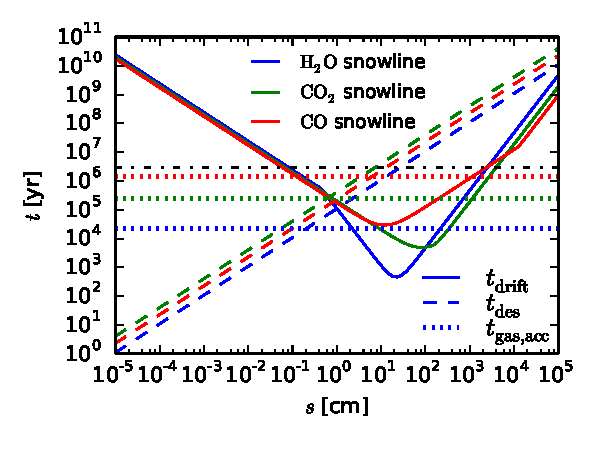
\includegraphics[width=0.5\textwidth]{../../figs/drift_timescales_betaS1_gas_acc_new.pdf}
%\vspace{-0.5in}
\caption{Relevant timescales for dynamical effects in the desorption process: $t_{\rm r, drift}$ (solid lines), $t_{\rm evap}$ (dashed lines) and $t_{\rm gas, acc}$ (dotted lines). The timescales are calculated at three representative locations in the disk: ... AU (blue lines), ... AU (green lines) and ... AU(red lines). The horizontal dashed line represents a typical disk lifetime of 3 Myr. Radial drift and gas accretion affect desorption in the regions where their respective timescales, i.e. $t_{\rm r, drift}$ and $t_{\rm gas, acc}$, are comparable to the desorption timescale $t_{\rm evap}$. \textbf{Figure belongs to section 2.4.} (\emgr{We will probably want to change the notation on the plot to $t_{des}$ instead of $t_{\rm evap}$ for consistency.})}  %  (See text for a description of evolution to yet higher masses.) 
\label{fig:timescales}
\end{figure}

\emgr{Calculate timescale for radial drift following Chiang \& Youdin (2010). Calculate desorption timescale following Hollenbach et al. (2009). Estimate gas accretion timescale for a given $\alpha$. Important: mention that, for simplicity and illustrative purposes, these calculations are performed for a passive disk. Show plot with the timescales as a function of particle size at different snowlines to show the regime in which drift matters}.



\section{Snowline Locations}

\begin{figure}[h!]
\centering
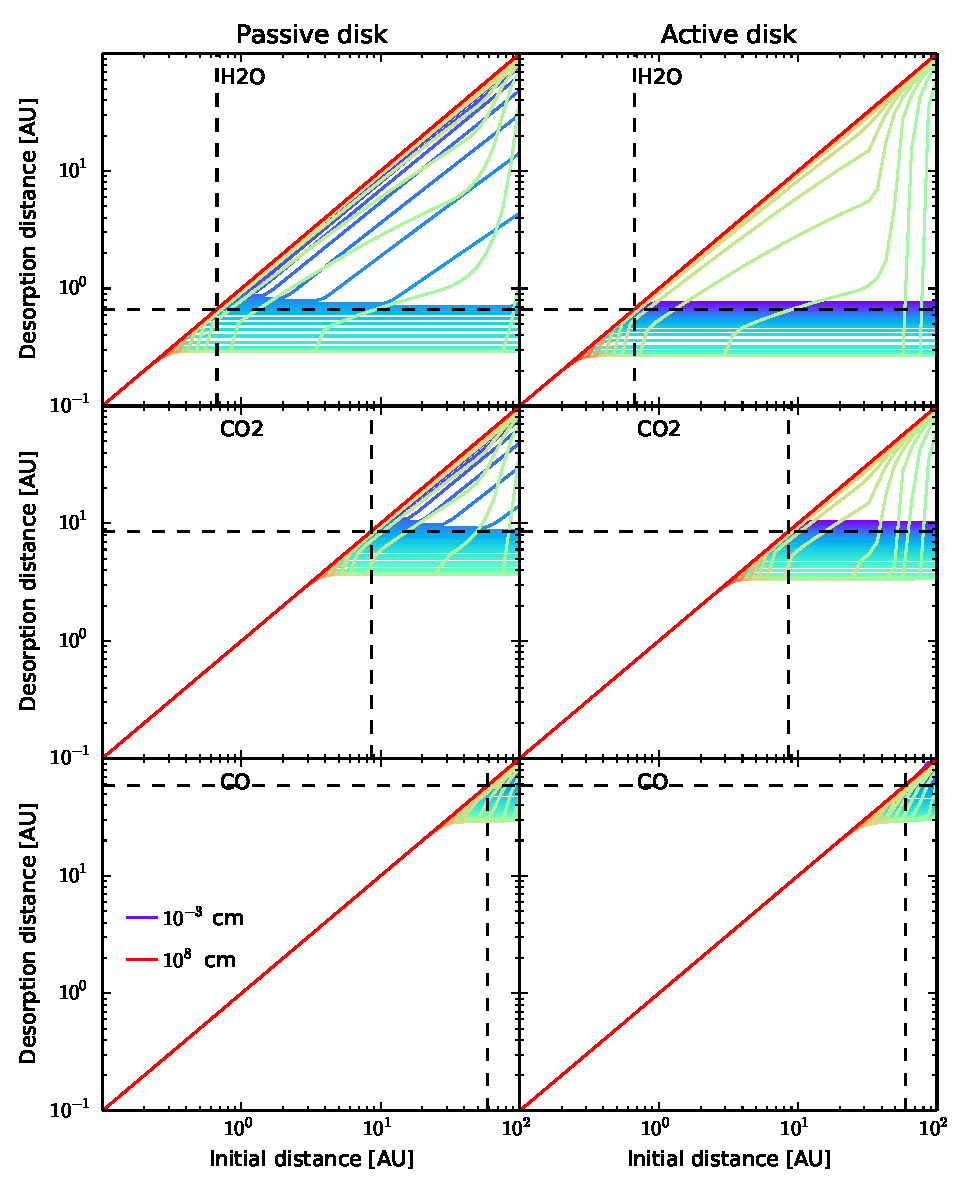
\includegraphics[width=0.5\textwidth]{../../figs/desorption_distance_passive_active.pdf}
%\vspace{-0.5in}
\caption{Desorption distance as a function of a particle's initial location in the disk, for a range of particle sizes, and for both a passive disk (left panels) and an active disk (right panels). The desorption distance is calculated for particles composed of H$_2$O (top panels), CO$_2$ (middle panels) and CO (bottom panels). The particle size increases from $10^{-3}$ cm to $10^8$ cm in a rainbow color scheme. For a range of particle sizes, the desorption distance is the same regardless of the particles' initial location. \textbf{Figure belongs to section 3.}}  %  (See text for a description of evolution to yet higher masses.) 
\label{fig:snowlines}
\end{figure}

\begin{figure}[h!]
\centering
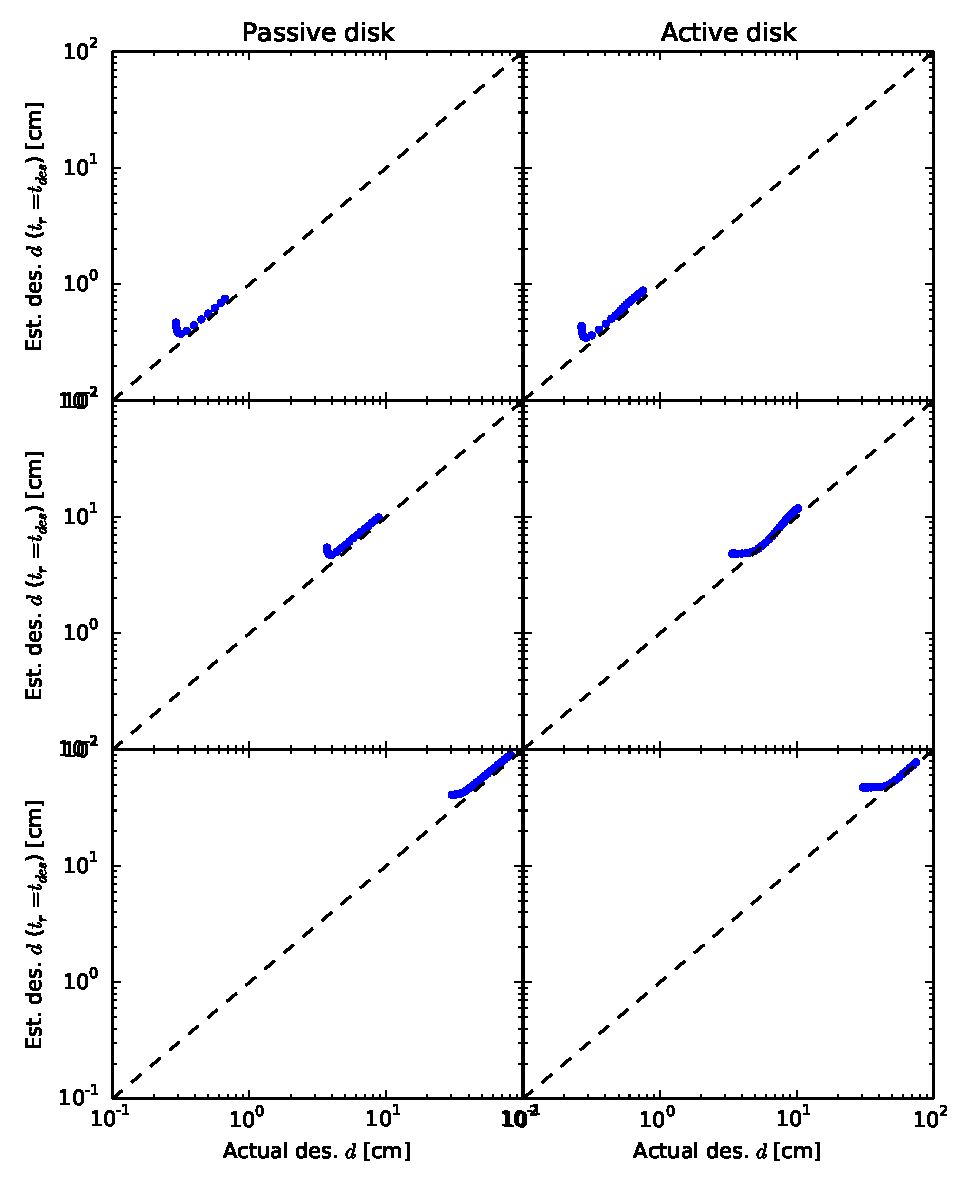
\includegraphics[width=0.5\textwidth]{../../figs/desorption_distance_actual_vs_estimated_passive_active.pdf}
%\vspace{-0.5in}
\caption{Desorption distance estimated from analytic calculations (see text) as a function of the desorption distance calculated numerically, for the range of particle sizes that desorb at a fixed distance regardless of initial location (see Figure \ref{fig:snowlines} and text). The estimate is performed for a passive disk (left panels) and an active disk (right panels).  The particles are composed of H$_2$O (top panels), CO$_2$ (middle panels) and CO (bottom panels). The analytic approximation is in good agreement with the numerical result for most cases. \textbf{Figure belongs to section 3.}}  %  (See text for a description of evolution to yet higher masses.) 
\label{fig:an_vs_actual}
\end{figure}

\begin{figure}[h!]
\centering
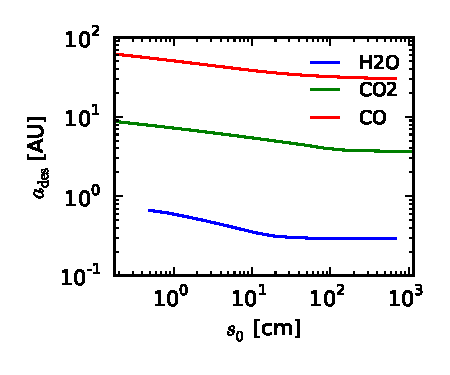
\includegraphics[width=0.5\textwidth]{../../figs/desorption_distance_vs_s.pdf}
%\vspace{-0.5in}
\caption{Desorption distance as a function of initial particle size, for the range of particles that desorb at a fixed distance regardless of initial location (see Figure \ref{fig:snowlines}). \textbf{Figure belongs to section 3.} \emgr{This is a figure that I'm not sure we should include, since it doesn't really provide that much useful inside. If we did include it though, there would be two panels both for the passive and the active disk. The caption is not complete since the active disk panel is not yet there.}}  %  (See text for a description of evolution to yet higher masses.) 
\label{fig:an_vs_actual}
\end{figure}

\emgr{Present the equation set that you are solving, $dr/dt=\dot{r}$, $ds/dt=...$. I don't think it is necessary to describe in detail the numerical method of solving the equations since it's pretty straightforward. Present the pretty rainbow plots side by side for passive and active disks, and highlight the differences. Insert the plots that shows that for the intermediate size particles, the desorption distance can be estimated analytically with good accuracy. Maybe also include the plot showing the desorption distance as a function of particle size, both for passive and active disk. Split into subsections?}


\section{Results for the C/O Ratio}

\begin{figure}[h!]
\centering
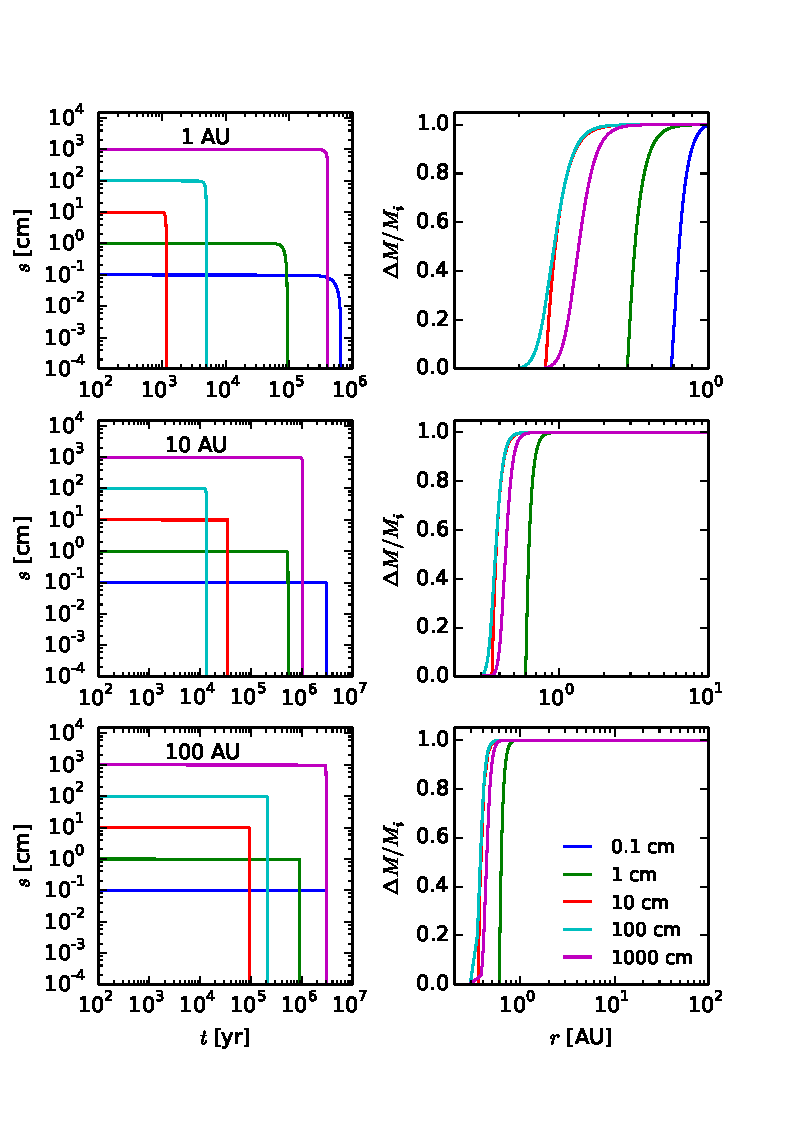
\includegraphics[width=0.5\textwidth]{../../figs/s_t_a.pdf}
%\vspace{-0.5in}
\caption{Left panels: size of desorbing H$_2$O particles as a function of time, for different initial particle sizes and for three initial locations in a passive disk: 1 AU (top left), 10 AU (middle left) and 100 AU (bottom left). Particles desorb almost instantaneously. Right panel: fractional mass lost by the desorbing particles as a function of the particle's location as it drifts, for different initial particle sizes, and at the same initial locations presented in the left panel. Particles lose most of their mass very close to the distance at which they fully desorb. \textbf{Figure belongs to section 4.}}
\label{fig:s_t_a}
\end{figure}

\begin{figure}[h!]
\centering
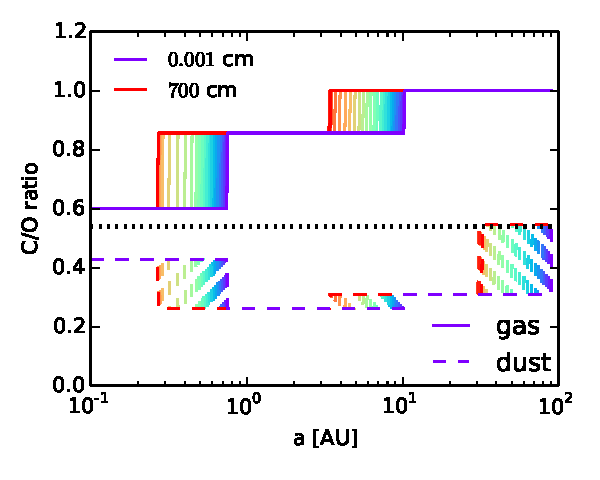
\includegraphics[width=0.5\textwidth]{../../figs/C_O_ratio_active_disk_many.pdf}
%\vspace{-0.5in}
\caption{C/O ratio in gas (solid lines) and in dust (dashed lines) for a passive disk (left panel \emgr{currently non-existent}) and for an active disk (right panel \emgr{currently just a single plot}), and for the range of particle sizes that desorb at a fixed distance regardless of their initial location in the disk. The particle size increases from 0.001 cm to 700 cm in a rainbow color scheme. The horizontal dotted line represents the stellar value of 0.54. The black lines (\emgr{currently non-existent}) represent the C/O ratio in gas (solid black line) and dust (dashed black line) for a static disk. The snowline location moves inward as the particle size increases. \textbf{Figure belongs to section 4.}}
\label{fig:CO_ratio}
\end{figure}

\begin{figure}[h!]
\centering
\includegraphics[width=0.5\textwidth]{lala}
%\vspace{-0.5in}
\caption{C/O ratios for different particle size distributions... \textbf{Figure belongs to section 4.} (\emgr{It will probably be a multi-panel plot, for different particle size distributions, for both passive and active disk, and perhaps at different times for the active disk. Not yet unsure how that figure will look like since I don't have the results yet, so I'll leave the figure caption open for now.})}
\label{fig:...}
\end{figure}

\emgr{Motivate the fact that we can calculate a sharp, fixed snowline for each particle size by inserting the plot that shows that particles desorb almost instantaneously at a fixed distance.  Then present the plots analogous to Fig. 1 in \"Oberg et al. (2011) for different particle sizes, based on the snowline locations obtained in the previous section, both for passive and active disk. Perhaps show it at different times in the gas disk evolution (i.e., not just at 3 Myr) for the active disk. Then assume a particle size distribution and show the interpolated result for the C/O ratio. Generalize the result using a transition disk (this part might also fit in the discussion section).}

%emgr{Present the flux equations used to keep track of the amount of C and O in gas and dust throughout the disk. Motivate the simplification of using a fixed particle sized, fixed timescale, and fixed desorption distance in the calculations by referring to the rainbow plot in the previous section and by inserting the plot that shows that particle desorb almost instantly at a fixed distance. Based on these assumptions, finally show the equivalent of Fig. 1 in \"Oberg et al. (2011) for different particle sizes, and at different times in the gas disk evolution (i.e., not just at 3 Myr) --- a multi-panel plot could be a good idea. Discuss the result, trends, etc. Ideally, have a final plot showing the results for a particle size distribution rather than for individual particles.}

\section{Discussion and Model Limitations}

\emgr{Present the diagram that shows all the effects that can modify snowline location. For model limitations, include: non-inclusion of turbulence, assumption of perfect spheres when in fact they may have cracks, particles composed of a single volatile when in reality they are likely to be mixed, etc. Discuss uncertainty of initial conditions and estimate how much they matter. ....}

\section{Summary and Future Work}

\emgr{Summarize results. Mention inclusion of $N_2$ as a first expansion. Mention the implementation of time-dependent chemical models in the drift calculation.}

\appendix
\section{...}

\emgr{Right now it's unclear to me what could go in an appendix, if anything. Maybe discuss a bit the algorithm to evolve $\Sigma_{\rm p}$ (although it is already explained in detail in the appendix of Birnstiel et al. 2010). Maybe show some example profiles of $\Sigma_{\rm p}$ at different times and for different particle sizes.}

\if\bibinc n
\bibliography{refs}
\fi

\if\bibinc y
\begin{thebibliography}
\end{thebibliography}
\fi


\end{document}